% Tamaño de letra.
\documentclass[12pt,titlepage]{article}
%\documentclass{article}

%------------------------------ Paquetes ----------------------------------

% Paquetes:

\usepackage[T1]{fontenc}

%Para comentarios multilínea.
\usepackage{verbatim}

% Para tener cabecera y pie de página con un estilo personalizado.
\usepackage{fancyhdr}

% Codificación UTF-8
\usepackage[utf8]{inputenc}

% Tipografía
\usepackage{palatino} % Esta es genial!
\linespread{1.05} % Palatino queda mejor con un poco más de interlineado.
%\usepackage{times} % Times New Roman.


% Castellano.
\usepackage[spanish]{babel}

% Tamaño de página y márgenes.
\usepackage[a4paper,left=2cm,right=2cm,headheight=16pt]{geometry}
%\usepackage[left=2cm,top=3cm,right=2cm,bottom=1cm,head=1.5cm,includefoot]{geometry}

% Para \href y \url
\usepackage[pdfauthor   ={Demian Ferreiro}%
           ,pdftitle    ={Trabajos Prácticos - Lenguajes Formales en Lisp}%
]{hyperref}
\hypersetup{
colorlinks=true,
linkcolor=black,
pdfborder= 0 0 0
}

% Gráficos:

% Para generar pdf.
\usepackage[pdftex]{graphicx}
\usepackage{float}
\usepackage{pdfpages}

% Para captions.
\usepackage{caption}

% Sarpadísima tipografía para listings y \texttt
\usepackage{inconsolata}

\usepackage{xcolor}

% Para ejemplos de código.
\usepackage{listings}
\lstset{language=Lisp
  ,basicstyle=\ttfamily\small % Usa inconsolata
  ,identifierstyle=\ttfamily
  ,keywordstyle=\color[rgb]{0,0,1}
  ,commentstyle=\color[rgb]{0.133,0.545,0.133}
  ,stringstyle=\color[rgb]{0.627,0.126,0.941}
  ,morekeywords={true,false}
  ,showstringspaces=false     % No muestra underscores en los espacios de los strings.
  ,backgroundcolor=\color{blue!10} % Un color suave de fondo (menos chocante que el frame=single)
  ,breaklines=false            % Wrappea las lineas automáticamente.
  ,belowskip=0pt               % Reduce el espacio entre un listing y el párrafo siguiente
  ,inputencoding=utf8
  ,literate={á}{{\'a}}1
           {é}{{\'e}}1
           {í}{{\'i}}1
           {ó}{{\'o}}1
           {ú}{{\'u}}1
           {´}{{$^{\prime}$}}1
           {`}{{$^{\backprime}$}}1
  %frame=single               % Un recuadro en los listings.
}

% Para fórmulas matemáticas.
\usepackage{amssymb,amsmath}

% Para pseudocódigo. Instalar texlive-science.
\usepackage{algorithmic}
\usepackage{algorithm}

% Para poder hacer \begin{Verbatim}[samepage=true]
\usepackage{fancyvrb}


% Son necesarios?
%\usepackage{float}

%------------------------------ ~paquetes ---------------------------------

%------------------------- Inicio del documento ---------------------------

\begin{document}

% ---------------------- Encabezado y pie de página -----------------------

% Encabezado: sección a la derecha.
% Pie de página: número de página a la derecha.

\pagestyle{fancy}
\renewcommand{\sectionmark}[1]{\markboth{}{\thesection\ \ #1}}
\lhead{}
\chead{}
\rhead{\rightmark}
\lfoot{}
\cfoot{}
\rfoot{\thepage}

% ---------------------- ~Encabezado y pie de página ----------------------

% -------------------------- Título y autor(es) ---------------------------

\title{Prolog}
\author{}

% -------------------------- ~Título y autor(es) --------------------------

% ------------------------------- Carátula --------------------------------

\begin{titlepage}

\thispagestyle{empty}

% Logo facultad.
\begin{center}

\includegraphics[scale=0.55]{./fiuba}\\
\textsc{\Large Universidad de Buenos Aires}\\[0.2cm]
\textsc{\Large Facultad de Ingeniería}\\[1.5cm]

% Título central.

\textsc{\large Lenguajes Formales (75.14)} \\[0.3cm]
% \textsc{\large Trabajos Prácticos} \\[0.5cm]

\rule{\linewidth}{0.5mm} \\[0.4cm]
{\huge \bfseries Trabajos Prácticos en Lisp} \\
%{\Large \bfseries Introducción al lenguaje y a la programación lógica}
\rule{\linewidth}{0.5mm} \\[1cm]

\vfill

\Large 
\begin{tabular}{lll}
Demian Ferrerio & 88443 & epidemian@gmail.com \\[0.5cm]
\end{tabular}

% Pie de página de la carátula.
{\Large \today}

\end{center}
\end{titlepage}

% ------------------------------- ~Carátula -------------------------------

% -------------------------------- Índice ---------------------------------

% Hago que las páginas se comiencen a contar a partir de aquí.
\setcounter{page}{1}

% Índice.
\tableofcontents
\newpage

% -------------------------------- ~Índice --------------------------------

% ----------------------------- Inicio del tp -----------------------------

\clearpage	

% Saca la indentación de los párrafos y añade un espacio entre cada uno.
\setlength{\parindent}{0pt}
\setlength{\parskip}{2ex plus 0.5ex minus 0.2ex}

% Luego del índice, links con color.
\hypersetup{
linkcolor=red
}

% Cosas Nuevas -----------------------------------------------------------------


\section{Introducción}

Los trabajos prácticos se realizaron usando SBCL\footnote{\url{http://www.sbcl.org/}} y Clisp\footnote{\url{http://www.clisp.org/}} como implementaciones de Common Lisp.

En las siguientes secciones se incluye el código fuente completo de cada ejercicio, una explicación de cómo se diseñó la solución y algunas pruebas para verificar su correcto funcionamiento.

\section{GPS}

El objetivo de este ejercicio es modelar calles e interescciones y diseñar un ``GPS'' que permita encontrar un camino para ir de un punto a otro.

\subsection{Grafo Simple}

Un grafo se modelará como una lista de elementos de la forma \lstinline|(a (b1 ... bn)|, donde \lstinline|a| y \lstinline|b1 ... bn| son nodos distintos y \lstinline|(a (b1 ... bn)| representa que existen aristas salientes de \lstinline|a| y entrantes en \lstinline|b1 ... bn|.

Por el momento, los nodos serán átomos. 
\begin{lstlisting}
; La representación del grafo no conexo:
;    a--c--f     
;    |    / \    h--i
;    b---d---g    \
;     \     /      j
;      `-e-´
(defparameter *grafo-simple* 
  '((a (b c)) (b (a d e)) (c (a f)) (d (b f g)) (e (b g)) (f (c d g)) 
    (g (d e f)) (h (i j)) (i (h)) (j (h))))
\end{lstlisting}

La variable global \lstinline|*grafo-simple*| es entonces un grafo no conexo y no dirigido que luego se usará para probar la función GPS.

Es importante notar que esta forma de modelar los grafos permite ahcer grafos dirigidos. Por ejemplo \lstinline|'((a (b)) (b (c)))| es un grafo dirigido donde se puede ir de \lstinline|a| hasta \lstinline|c| pero no al revés. Esto se usará luego para modelar calles de mano única.

\subsection{Encontrar un Camino}

Para encontrar un camino será necesario comparar nodos. Para ello, conviene hacer una función que verifique si dos nodos son iguales.
\begin{lstlisting}
(defun nodos-iguales (a b)
  (or (eql a b)))
\end{lstlisting}
Por ahora con derivar a \lstinline|eql| alcanza, pues los nodos son simples átomos. Más adelante se redefinirá esta función para poder comparar esquinas de calles.

También será necesario encontrar, para un nodo dado, sus vecinos:
\begin{lstlisting}
; Devuelve los nodos vecinos de un nodo en un grafo dado.
(defun vecinos (nodo grafo)
  (cadr (find nodo grafo :key 'car :test 'nodos-iguales)))
\end{lstlisting}
Nótese que se está usando la función \lstinline|nodos-iguales| para comparar nodos.

Para probar que esta función anda correctamente, se puede ejecutar en el ambiente interactivo de Lisp:
\begin{lstlisting}
> (vecinos 'f *grafo-simple*)
(C D G)
\end{lstlisting}

Con esto ya se puede hacer una primer implementación del GPS:
\begin{lstlisting}[basicstyle=\ttfamily\footnotesize]
; Devuelve un camino que conecta los nodos inicio y fin en un grado dado, o nil 
; en caso de no existir camino alguno.
(defun gps (inicio fin grafo &optional (trayectorias (list (list inicio))))
  (if (null trayectorias) nil
      (if (nodos-iguales (caar trayectorias) fin)
          (reverse (car trayectorias))
          (gps inicio fin grafo 
               (append (expandir-trayectoria (car trayectorias) grafo)
                       (cdr trayectorias))))))

; Devuelve todas las posibles "expansiones" de una trayectoria dada agregando 
; los vecinos del primer nodo que aún no formen parte de la misma.
(defun expandir-trayectoria (trayectoria grafo)
  (mapcar (lambda (vecino) (cons vecino trayectoria))
          (set-difference (vecinos (car trayectoria) grafo) trayectoria)))

\end{lstlisting}

Este algotritmo hace una búsqueda en profundidad de las trayectorias posibles hasta encontrar alguna que sea una camino que conecto los nodos \lstinline|inicio| y \lstinline|fin|. La función \lstinline|expandir-trayectoria| devuelve todas las trayectorias posibles que resulten de tomar un nodo vecino del primer nodo que aún no forme parte de la trayectoria dada; puede devolver \lstinline|nil| cuando no quedan más caminos por tomar para una trayectoria dada, y en ese caso es que se descartará esa trayectoria y se continuará expandiendo la siguiente en la función \lstinline|gps| hasta cubrirlas todas.

Algunas puebras:
\begin{lstlisting}
> (gps 'c 'c *grafo-simple*)
(C)
> (gps 'c 'e *grafo-simple*)
(C A B D F G E)
> (gps 'c 'i *grafo-simple*)
NIL
\end{lstlisting}

Se puede observar que el camino encontrado entre los nodos \lstinline|c| y \lstinline|e| no es el más corto posible, pero es una solución válida.

\subsection{Camino Mínimo}

Encontrar un camino mínimo a partir de las funciones ya definidas resulta sencillo:
\begin{lstlisting}[basicstyle=\ttfamily\footnotesize]
; Devuelve un camino mínimo que conecta los nodos inicio y fin en un grado dado,
; o nil en caso de no existir camino alguno.
(defun gps-min (inicio fin grafo &optional (trayectorias (list (list inicio))))
  (if (null trayectorias) nil
      (or (reverse (find fin trayectorias :key 'car :test 'nodos-iguales))
          (gps-min inicio fin grafo
                   (mapcan (lambda (tr) (expandir-trayectoria tr grafo))
                           trayectorias)))))
\end{lstlisting}

Este algoritmo hace, en vez de una búsqueda en profundidad, una busqueda en anchura de las trayectorias posibles, es por eso que cuando encuentra una solución, ésta tiene que ser mínima. En cada llamada recursiva se checkea si alguna de las trayectorias es solución y en caso de que ninguna lo sea se vuelve a llamar recursivamente a \lstinline|gps-min| pasándole todas las trayectorias expandidas.

Ejemplo de uso:
\begin{lstlisting}
> (gps-min 'c 'e *grafo-simple*)
(C A B E)
\end{lstlisting}

Este camino sí es mínimo :)

\subsection{Calles}

Para hacer un grafo que represente un mapa de calles, los nodos deberán representar intersecciones entre calles. Para ello, pasarán de ser simples átomos a ser una lista de dos strings que serán los nombres de las calles que se intersectan en ese nodo. Por ejemplo \lstinline|("Paseo Colon" "Independencia")| es un nodo que representa la intersección entre las calles Paseo Colón e Independencia.

La definición de \lstinline|nodos-iguales| cambiará acorde a la neuva definición de nodo:
\begin{lstlisting}
; Verifica si dos nodos a y b son iguales.
(defun nodos-iguales (a b)
  (or (equalp a b) 
      (and (listp a) (listp b) (equalp a (reverse b)))))
\end{lstlisting}

Esto es así porque se desea que \lstinline|("Paseo Colon" "Independencia")| y \lstinline|("Independencia" "Paseo Colon")| representen la misma intersección.

Para hacer las pruebas, se modelará parte de las calles aledañas a la Facultad de Ingeniería:
\begin{figure}[H]
\begin{center}
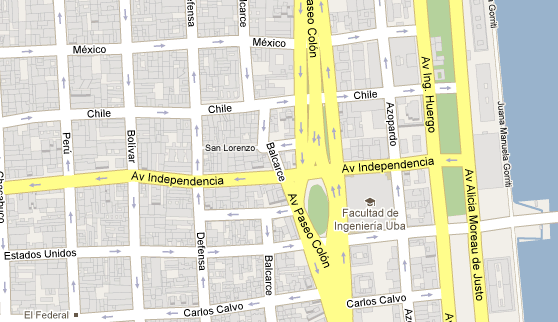
\includegraphics[width=10cm]{mapa.png}
\caption{Mapa de la zona donde se ubica la Facultad de Ingeniería sacado de Google Maps.}
\end{center}
\end{figure}

Para hacer más sencilla la tarea de armar el grafo de calles, se numerarán las intersecciones que se desean modelar:
\begin{figure}[H]
\begin{center}
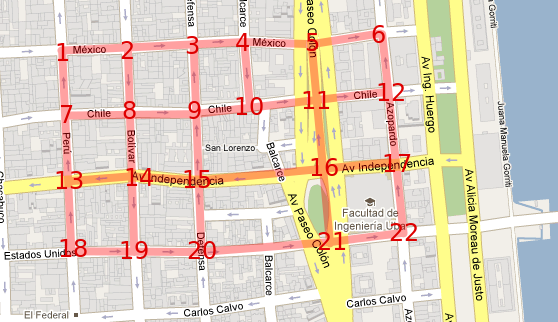
\includegraphics[width=10cm]{mapa-numerado.png}
\caption{Enumeración de las intersecciones a modelar.}
\end{center}
\end{figure}

El grafo de estas calles se cargará en una variable global \lstinline|*mapa-facu*|, que se define de la siguiente manera:
\begin{lstlisting}[basicstyle=\ttfamily\footnotesize]
(defparameter *mapa-facu*
  (let* ((mx "Mexico") (ch "Chile") (in "Independencia") (eu "Estados Unidos") 
         (pe "Peru") (bo "Bolivar") (de "Defensa") (ba "Balcarce") 
         (pc "Paseo Colon") (az "Azopardo"))
    (crear-grafo (append (crear-calle mx (list pe bo de ba pc az))
                         (crear-calle ch (list pe bo de ba pc az))
                         (crear-calle in (list az pc de bo pe))
                         (crear-calle eu (list pe bo de pc az))
                         (crear-calle pe (list eu in ch mx))
                         (crear-calle bo (list mx ch in eu))
                         (crear-calle de (list eu in ch mx))
                         (crear-calle ba (list mx ch))
                         (crear-calle pc (list mx ch in eu))
                         (crear-calle pc (list eu in ch mx))
                         (crear-calle az (list eu in ch mx)))))) 
\end{lstlisting}

Las funciones \lstinline|crear-grafo| y \lstinline|crear-calle| pueden encontrarse el código fuente del programa (\ref{lst:gps}). Lo que es importante saber es que el grafo creado respeta las manos de las calles, que son de mano única.

Gracias a que las calles son de mano única, los caminos mínimos no son tan directos:
\begin{lstlisting}[basicstyle=\ttfamily\footnotesize]
> (gps-min '("Balcarce" "Mexico") '("Estados Unidos" "Bolivar") *mapa-facu*)
(("Balcarce" "Mexico") ("Mexico" "Paseo Colon") ("Paseo Colon" "Chile")
 ("Paseo Colon" "Independencia") ("Independencia" "Defensa")
 ("Independencia" "Bolivar") ("Bolivar" "Estados Unidos"))
\end{lstlisting}

\subsection{Imprimir Camino}

La función \lstinline|imprimir-camino| es útil para hacer más legibles los caminos encontrados. Su definición puede encontrarse en el código fuente del programa (\ref{lst:gps}). Por ahora, nos conformamos con una prueba:
\begin{lstlisting}[basicstyle=\ttfamily\footnotesize]
> (imprimir-camino (gps-min '("Balcarce" "Mexico") '("Estados Unidos" "Bolivar") 
*mapa-facu*))
Tomar "Mexico" hasta "Paseo Colon"
Tomar "Paseo Colon" hasta "Independencia"
Tomar "Independencia" hasta "Bolivar"
Tomar "Bolivar" hasta "Estados Unidos"
\end{lstlisting}

\subsection{Código fuente}

\lstinputlisting[basicstyle=\ttfamily\footnotesize,label=lst:gps,caption={gps.lisp}]{../gps/gps.lisp}

\section{Intérprete TLC}
\section{Intérprete C}
\section{N Reinas}

% ------------------------------ Fin del tp -------------------------------

\end{document} 

%---------------------------- Fin del documento ---------------------------
